\documentclass[dvisvgm,tikz,border=4pt]{standalone}
\usepackage{amsmath,amssymb}

\usetikzlibrary{arrows.meta,positioning,automata,shapes,shapes.misc,calc,decorations.pathmorphing,decorations.markings,angles,quotes,patterns,mindmap,matrix,knots,hobby,trees}
\tikzset{->-/.style={decoration={markings, mark=at position 0.5 with {\arrow{Stealth}}}, postaction={decorate}}}
\begin{document}
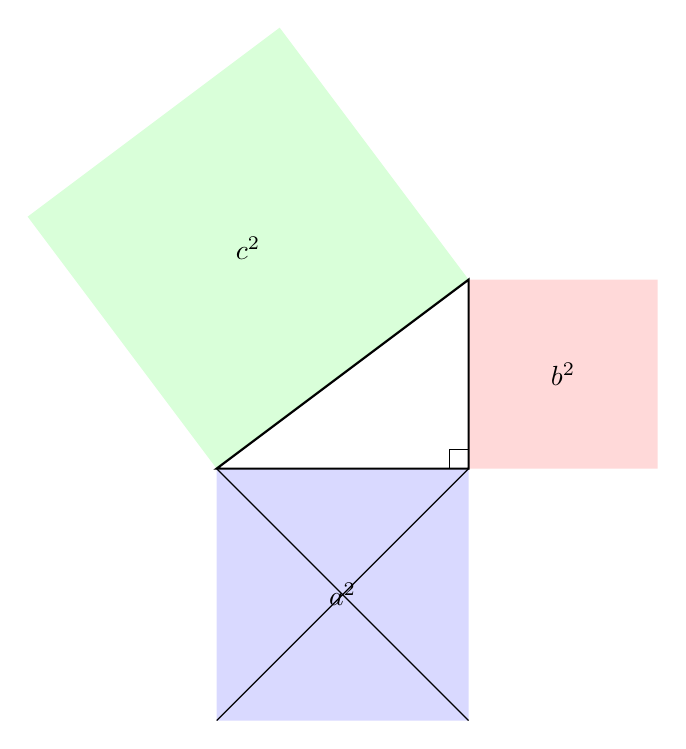
\begin{tikzpicture}[scale=0.8]
\coordinate (A) at (0,0); \coordinate (B) at (4,0); \coordinate (C) at (4,3);
\fill[blue!15] (A) -- (B) -- (4,-4) -- (0,-4) -- cycle;
\fill[red!15] (B) -- (C) -- (7,3) -- (7,0) -- cycle;
\fill[green!15] (A) -- (C) -- (1,7) -- (-3,4) -- cycle;
\draw[thick] (A) -- (B) -- (C) -- cycle;
\draw (A) -- (4,-4) (B) -- (0,-4);
\draw (3.7,0) |- (4,0.3);
\node at (2,-2) {$a^2$}; \node at (5.5,1.5) {$b^2$}; \node at (0.5,3.5) {$c^2$};
\end{tikzpicture}
\end{document}
